\section{Categorical and continuous data plots}
	A dataset is said to be \emph{categorical} if its independent variable takes one of a small, discrete set of labels (e.g. the day of the week, the floor number of a skyscraper), and \emph{continuous} if its independent variable can take any value within a range (e.g. time, angle, or magnetic field strength). The choice of plot type should follow from which of these two kinds of variable is being plotted, not from visual preference alone.
	
	\subsection{Column plots}
		In a \emph{column plot}, each category is represented as a vertical bar whose height is proportional to a summary value (such as a mean, a total or a count). %In a \emph{bar plot}, the idea is the same except that it is drawn using horizontal bars. Both types of plots are appropriate when the independent variable is categorical.
		
		\subsubsection{Creating a column plot in Origin}
			As a demonstration, we will create a column plot using the file named \texttt{mean-data.csv}, which has recorded the average temperature, humidity and pressure data for five weeks.
			\begin{enumerate}[I.]
				\item We open the CSV file as described in the previous unit. To create the column plot for the mean temperatures for five weeks, first we select the entire column by clicking on the column name.
				\begin{figure}[h!]
					\centering
					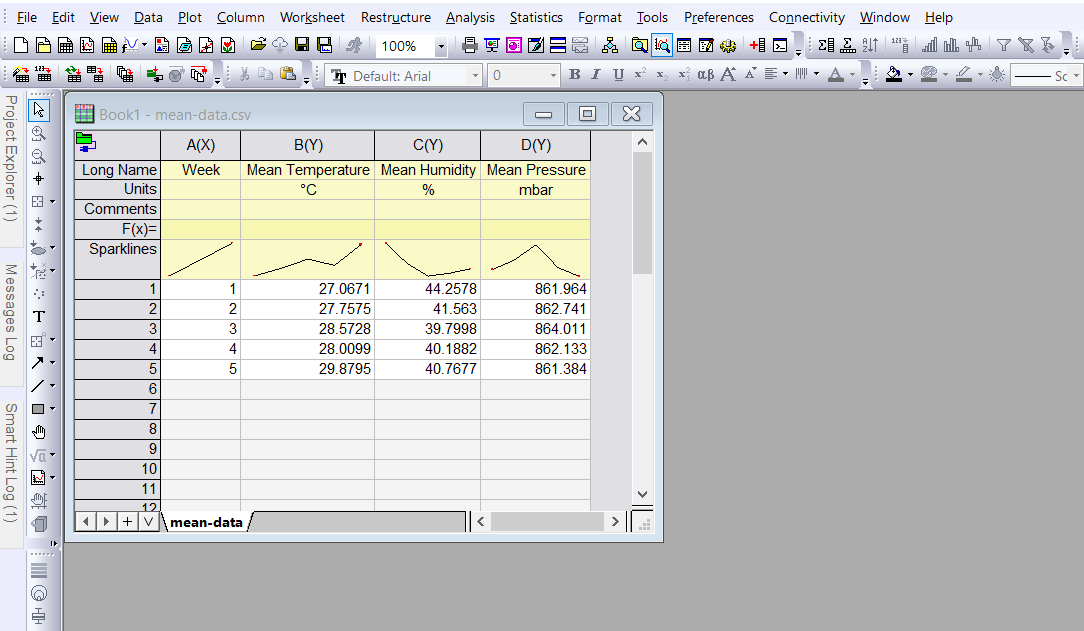
\includegraphics[width=0.5\textwidth]{figures/fig_column-bar-01.png}
					\hfill
					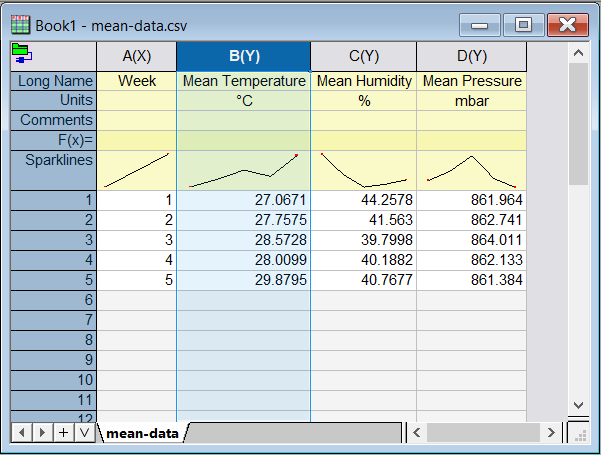
\includegraphics[width=0.45\textwidth]{figures/fig_column-bar-single-01.png}
				\end{figure}
				
				\item From the main menu, we click \verb|Plot > Bar, Pie, Area|, and then click \verb|Column|.
				\begin{figure}[h!]
					\centering
					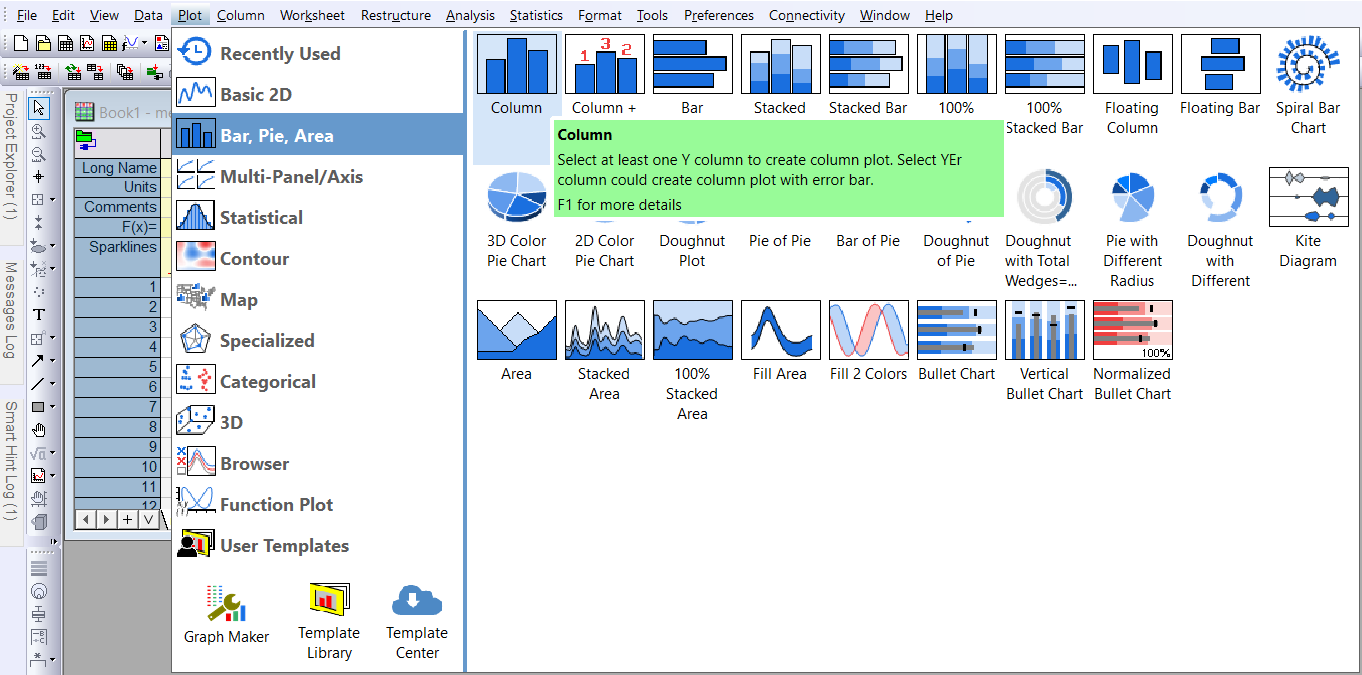
\includegraphics[width=0.55\textwidth]{figures/fig_column-bar-single-02.png}
				\end{figure}
				
				\item This produces a rudimentary column plot with default settings.
				\begin{figure}[h!]
					\centering
					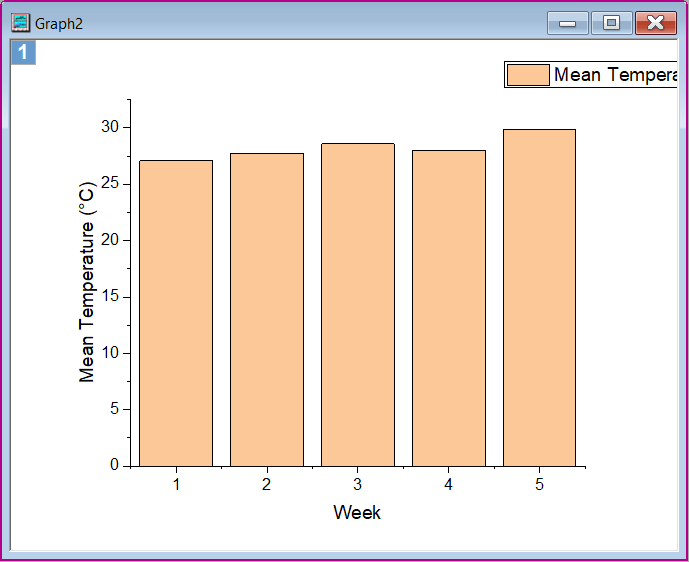
\includegraphics[width=0.4\textwidth]{figures/fig_column-bar-single-03.png}
				\end{figure}
				
				\item Because this is a column plot of only the mean temperature, we can click on the legend at the top right and press the delete button to remove it.
				\begin{figure}[h!]
					\centering
					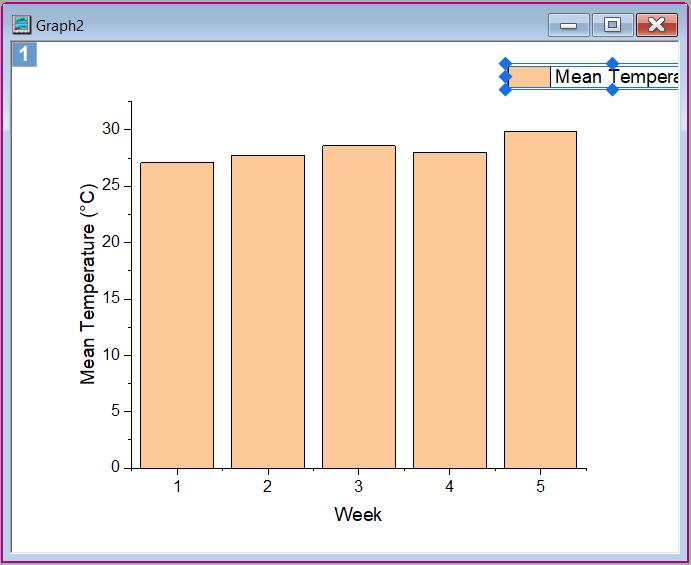
\includegraphics[width=0.4\textwidth]{figures/fig_column-bar-single-04.png}
					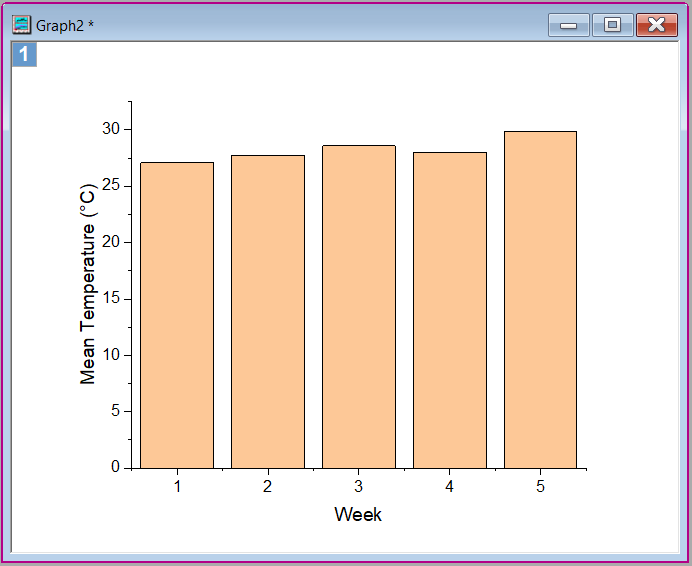
\includegraphics[width=0.4\textwidth]{figures/fig_column-bar-single-05.png}
				\end{figure}
				
				\item Because the column bars are about similar heights, we are unable to notice significant differences between them if we plot them from zero at the bottom. So we need to change the scale of the $y$-axis values in a manner such that their differences become more pronounced.
				
				To do so, we click on any of the $y$-tick labels and then click the \verb|Open Properties Dialog| logo.
				\begin{figure}[h!]
					\centering
					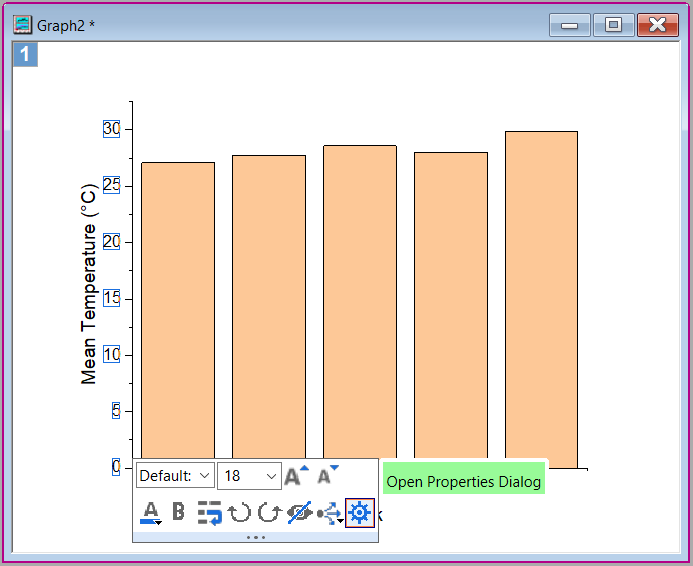
\includegraphics[width=0.4\textwidth]{figures/fig_column-bar-single-06.png}
				\end{figure}
				
				\item In the \verb|Properties| dialog, we click on the \verb|Scale| tab and approximately set the following values as \verb|From = 25|, \verb|To = 32|, so as to ensure that the $y$-axis spans the values from 25 to 32.
				
				We also set the major ticks as\vspace{-2ex}
				\begin{verbatim}
					Type = By Increment
					Value = 2
				\end{verbatim}\vspace{-3ex}
				and the minor ticks as\vspace{-2ex}
				\begin{verbatim}
					Type = By Counts
					Value = 1
				\end{verbatim}
				\begin{figure}[h!]
					\centering
					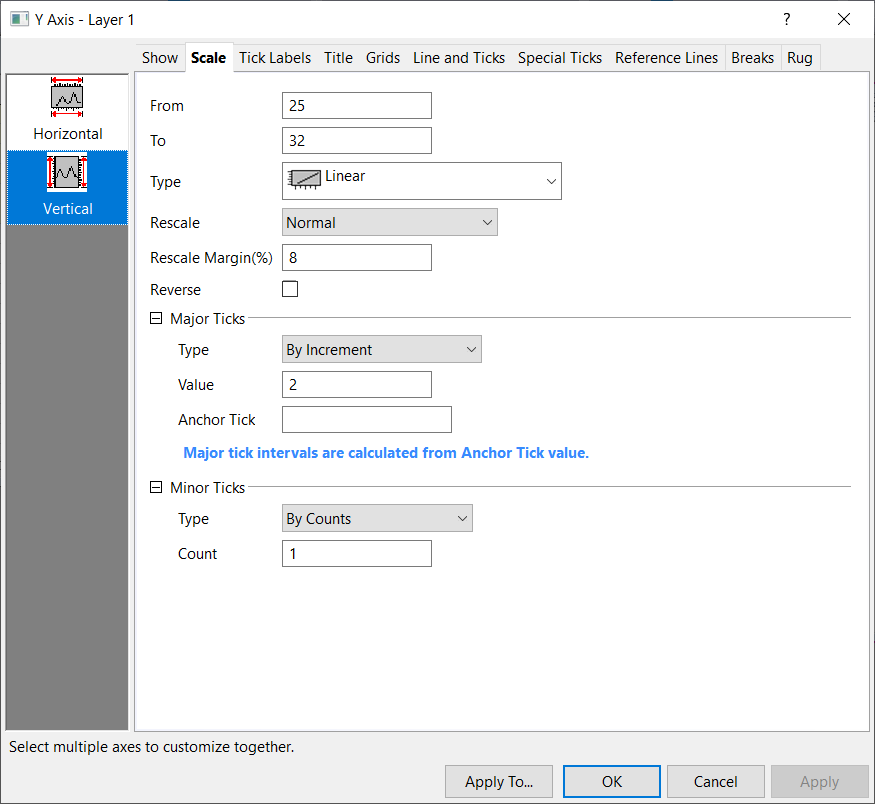
\includegraphics[width=0.5\textwidth]{figures/fig_column-bar-single-07.png}
					\hfill
					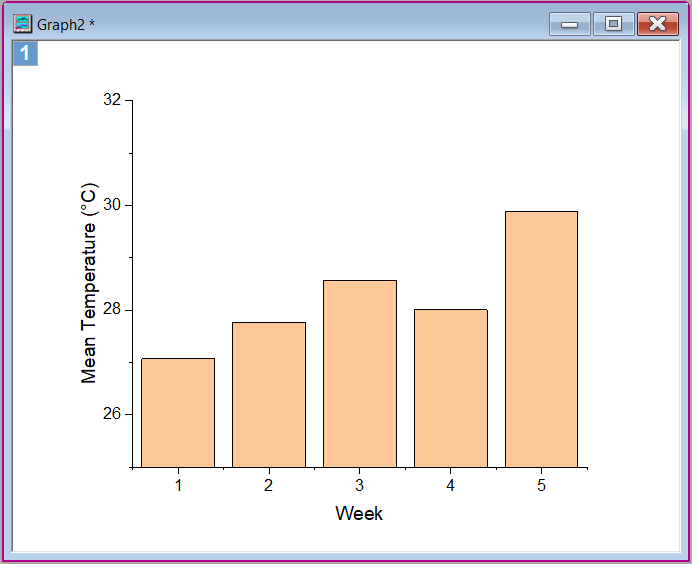
\includegraphics[width=0.45\textwidth]{figures/fig_column-bar-single-08.png}
				\end{figure}
				This shows much more discernible differences between the mean temperatures.
				
				\item Finally to place the graph within a rectangular bounding box, first we need to enable opposite axes by clicking on any of the axes lines, say the $x$-axis line, and then clicking on the \verb|Show Opposite Axis| button, so that an identical axis appears at the top. Then we click on the new axis at the top, then click on \verb|Axis Type| button and lastly click on \verb|None|.
				\begin{figure}[h!]
					\centering
					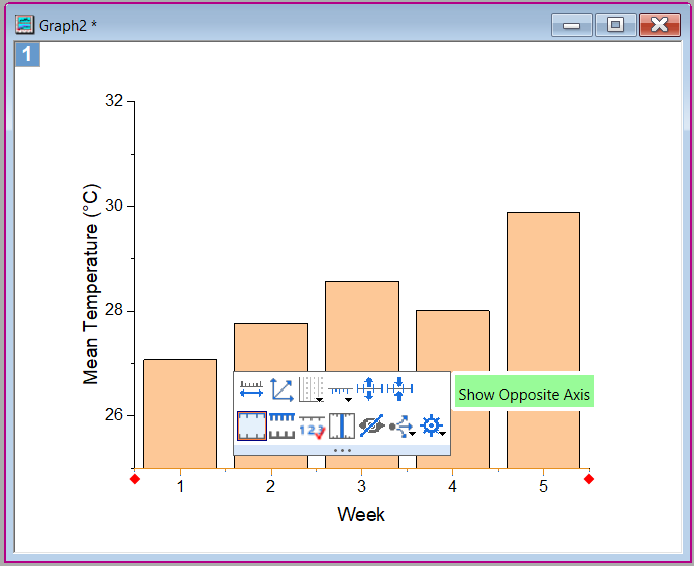
\includegraphics[width=0.45\textwidth]{figures/fig_column-bar-single-09.png}
					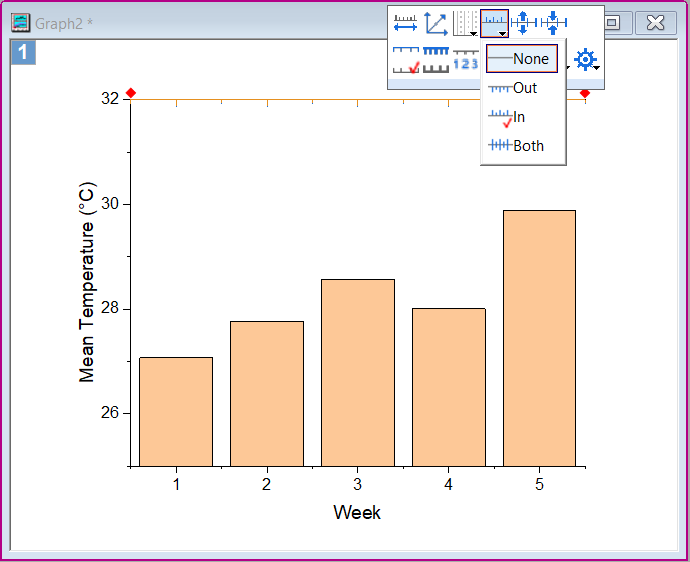
\includegraphics[width=0.45\textwidth]{figures/fig_column-bar-single-10.png}
				\end{figure}
				
				\newpage
				\item We repeat the same process for the $y$-axis as well to finally obtain the required column plot within a bounding box.
				\begin{figure}[h!]
					\centering
					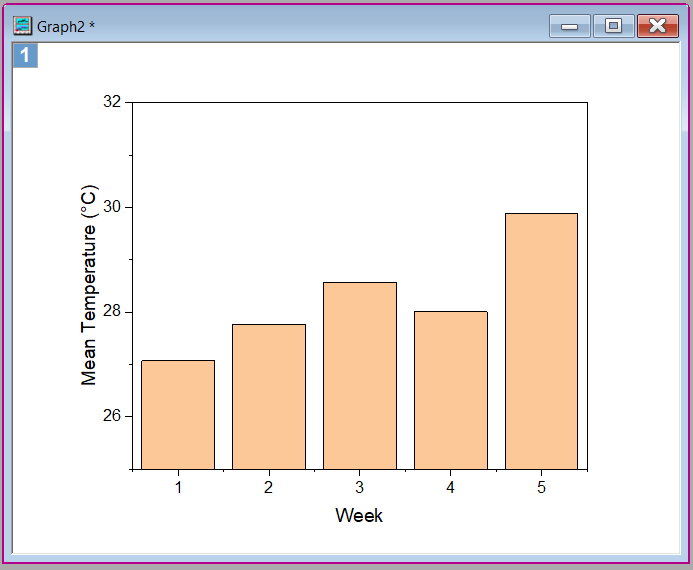
\includegraphics[width=0.5\textwidth]{figures/fig_column-bar-single-11.png}
				\end{figure}
			\end{enumerate}
	
	\subsection{Line plots}
		A \emph{line plot} connects successive data points with straight (or smoothed) line segments. It is the standard choice for a continuous independent variable, most commonly time. It should not be used for categorical data, since a line drawn between two unrelated categories implies a continuity between them that does not exist.
	
	\subsection{Pie charts}
		A \emph{pie chart} represents each category's share of a whole as a wedge of a circle, with wedge angle proportional to that category's proportion of the total. Pie charts are appropriate only for categorical data that sums to a meaningful whole, and are best limited to a small number of categories (three to five); beyond this, a column chart is usually clearer.
	
	\subsection{Area plots}
		An \emph{area plot} is a line plot with the region between the line and the axis filled in. It is used, in place of an ordinary line plot, when the magnitude of a continuously-varying quantity is the point of emphasis, or when several such quantities are to be compared by their relative contribution to a stacked total.
	
	\subsection{Scatter plots}
		A \emph{scatter plot} represents each observation as an individual point, with no line joining successive points. It is the correct choice when the relationship between two continuous variables is of interest, rather than the trend of one variable against time. A scatter plot is particularly used when there is no reason to assume the points are ordered or continuous in the underlying physical process.